\section{Neurona biológica}
\subsection{La neurona}
La neurona es un tipo de célula perteneciente al sistema nervioso central, estas se comunican tanto por señales eléctricas como por señales químicas.Cada neurona tiene un cuerpo celular (\textbf{soma}) que contiene un núcleo y otros componentes celulares, también se compone de una zona de recepción denominada \textbf{dendritas} y una zona de emisión conocida como \textbf{axón}. Pensemos en la neurona como toda una compuerta, por un lado esta el cuerpo de la de una neurona típica, en la dendrita tenemos una mezcla de neurotransmisores, y los iones que pueden moverse a través de la membrana. La forma en que recibe/ intercambia información va a ser mediante sustancias químicas y iones que están intercambiando, entre la parte de afuera y de adentro de la neurona. Particularmente en las dendritas, se tienen terminaciones que se pueden conectar con otras neuronas y de esta manera permitir el paso de información. Lo que sucede en estas conexiones es un intercambio químico que produce cambios de polaridad en la membrana. En el interior de la neurona hay una cierta carga eléctrica, así como en el exterior (el líquido de afuera) hay otra carga eléctrica, es decir, hay una \textbf{diferencia de potencial} entre el interior y el exterior de la neurona, por eso se dice que la membrana en sí misma tiene una carga eléctrica. Dado que es porosa, esta membrana  va a estar intercambiando partículas con el exterior, esto va a hacer que la polarización de esta membrana cambie, si en algún momento la diferencia de potencial neta rebasa un cierto umbral.

\begin{figure}[h]
 \centering
 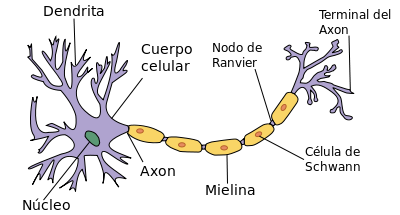
\includegraphics[scale=0.5]{../Figuras/neuronaPartes.png}
 \caption{Neurona, Acracia, 14 January 2007, Wikimedia Commons, \url{https://commons.wikimedia.org/wiki/File:Neurona.svg}, Creative Commons Attribution-ShareAlike 2.5 Generic}
 \label{fig:neuronaP}
\end{figure}


Ahora la neurona está recibiendo estos cambios, a partir de todas sus dendritas, cada cambio se está sumando en su cuerpo, en el \textbf{cono sónico} (uno de los nodos, en la representación de los diagramas de las neuronas artificiales) se va a estar sumando, la contribución de todos los efectos de cambios de potencial, si se rebasa un cierto valor umbral, en ese momento desencadena que la diferencia de potencial se propague, de aquí hasta la parte final del axón. Después vamos a tener un \textbf{período refractario} donde empieza a cambiar el potencial entre el cono sónico y el axón de la neurona, que va a transmitir una especie de disparo eléctrico en ese momento y va a “dejar de funcionar” durante un breve momento, para que la señal solamente pueda viajar hacia el axón, se va a quedar quieta un rato la neurona y vamos a notar un cambio muy violento en el voltaje, que se va recorriendo a lo largo de todo el axón. Tenemos unas células, que forman nodos que van cubriendo al axón para evitar que se pierda la señal, estos nodos recargan otra vez la señal y permite que avance, al siguiente nodo, donde se recarga  nuevamente y avance, hasta que logre llegar al final de axón.

Este trayecto puede ser de una neurona a unas pocas neuronas vecinas, hasta unos cuantos metros (ej. esta podría estar en la médula espinal y el axón llegar hasta el dedo), Cuando la señal llega a la colita de la axón, hay varias terminales que van a reaccionar ante el cambio de electricidad, mediante la liberación de unas vesículas, que contienen \textbf{neurotransmisores}.


\subsection{Elementos de las neuronas y tipos}

Elementos en la transmisión de señales:

\begin{itemize}
\item \textbf{Neurotransmisores:} son los mensajeros químicos que se comunican entre neuronas adyacentes; La liberación de neurotransmisores de una neurona ayudará a despolarizar o hiperpolarizar (aumentar la magnitud de la carga) la neurona adyacente, lo que hará que sea más o menos probable que ocurra un potencial de acción en la siguiente neurona.
  
\item \textbf{Impulsos eléctricos:} sucede cuando, ya se acumularon demasiadas señales, entonces a través de las dendritas la neurona, puede disparar un impulso eléctrico, a través del axón, que va a provocar que en su terminal libere más químicos, estos químicos son los hacen los efectos pequeños en cada uno de los cuerpos de las neuronas y el disparo eléctrico es como ya una señal mucho más intensa, para comunicarse con neuronas vecinas, con esto le están pasando información, esto se repite en varias ocasiones y cuando acumula suficiente, dispara, ese va a ser el impulso eléctrico. Se caracteriza por que son potenciales de acción que son, cambios de voltaje que van a ir ocurriendo a lo largo del axón.
 
\item \textbf{Plasticidad:} en el cerebro las neuronas pueden cambiar de manera permanente,   perder canales (que permiten el intercambio de nuevos transmisores sin impulsos eléctricos), formar más canales o incluso pueden crear protuberancias. Por ejemplo, cuando un cerebro aprende está transformando su arquitectura, es decir, los aprendizajes de largo plazo, modifican el cerebro y en consecuencia va a pensar y reaccionar distinto, que antes del aprendizaje.
\end{itemize}

Tipos:

\begin{itemize}
\item \textbf{Neuronas sin axones}, nunca dispara pero si tiene intercambios de neurotransmisores en las dendritas   
\item \textbf{Neuronas bipolares}, tienen dos axones. 
\item \textbf{Neurona unipolar}, solamente hay una conexión entre el cuerpo y el axón pero el axón tiene dos ramas, cuando dispare va a disparar hacia los dos lados, haciendo llegar su señal a diferentes regiones. 
\item \textbf{Neurona multipolar}, la más conocida, empieza con un cuerpo con dendritas y luego un largo axón que va a terminar con varias terminaciones axónicas. 
\end{itemize}

Otras situaciones 

Llega a pasar que no solamente se conectan axones con dendritas, también un axón se puede llegar a conectar directamente con el cuerpo de una neurona o axones se conectan con axones.

Cuando modelamos redes neuronales lo típico es modelar, una neurona con dendritas, su disparo y su axón, que se conecta con las siguientes dendritas,
pero aquí ya estamos viendo que la naturaleza nos dice que hay que pensar más y plantear cómo hacer la representaciones de estas conexiones que nos presenta la naturaleza, un poco diferente pero tal vez con resultados más satisfactorios.


\subsection{Sinapsis}
Aquí veremos cómo es que una neurona recibe o transmite información a otras neuronas. Para un solo disparo están participando un montón de elementos. 

\begin{figure}[h]
 \centering
 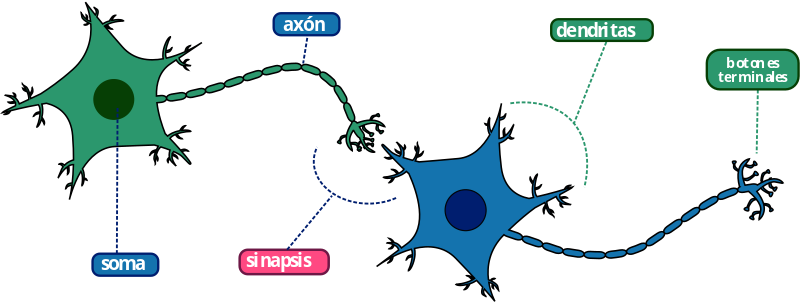
\includegraphics[scale=0.5]{../Figuras/Part_of_neurons_in_Spanish.png}
 \caption{Part of neurons in Spanish, Dana Scarinci Zabaleta, 24 February 2019, Wikimedia Commons, \url{https://commons.wikimedia.org/wiki/File:Part_of_neurons_in_Spanish.svg}, OpenStax, CC0}
 \label{fig:sinapsisN}
\end{figure}

Distingamos entre dos tipos de canales en las membranas: 
\begin{itemize}
\item \textbf{Receptores de neurotransmisores} que van a participar en las sinapsis \underline{químicas} en la zona de las dendritas.
\item \textbf{Canales iónicos} son quienes provocan las diferencias de carga entre el exterior y el interior de la neurona y participan en las sinapsis \underline{eléctricas} (conocido como la brecha sináptica)
\end{itemize}

La neurona está recibiendo un montón de señales por la liberación de neurotransmisores tanto de sus vecinos, como lo que ella misma va intercambiando, 
una vez que están generando el efecto completo de cambiar la polarización de
la red,  van a provocar que la neurona haga un disparo eléctrico. En el cuerpo están estos intercambios de iones que se suman en el cono sónico, empieza a viajar a través del axón,  en las vainas de mielina (donde se refuerza la señal). 
Aquí hacemos mención por primera vez de los iones positivos: sodio y potasio, estos iones lo que hacen es, que \emph{la membrana tenga una cierta carga la mayor parte del tiempo}. Cuando salen 3 sodios entran 2 potasios, entonces siempre hay más positivos afuera que en el interior de la neurona, es decir, por lo general  \emph{tiene una carga más negativa que su entorno}. Cuando ocurre un disparo de la neurona y se da el cambio de polarización en la membrana, se abren sus poros/ canales. El hecho que los canales abran o cierren depende de varios cambios que puedan estar ocurriendo alrededor de la neurona, en particular los que transmiten el disparo eléctrico, reaccionan ante el cambio de potencial que ocurrió en la membrana de la neurona. A esto le llaman la \textbf{conducción a saltos}, la señal va pasando por los nodos de Rainvier, se refuerza y pasa por los canales ionicos ya abiertos, hasta finalmente llegar a la sinapsis. Ahora lo que ocurre al final del recorrido es que, el cambio de electricidad otra vez provoca que unas vesículas, que están en el interior de la neurona,  que contienen a los neurotransmisores, se peguen a las sinapsis y se liberen esos neurotransmisores. 

Entonces la información le va a llegar a la neurona vecina, en la forma de neurotransmisores que fueron liberados (en lo que sea que lo haya recibido, típicamente son dendritas, pero podría ser su cuerpo o su axón), eso es lo que va a percibir la otra neurona y otra vez esta otra neurona va a empezar a sumar los efectos de estos neurotransmisores, para que en algún momento decida a lo mejor disparar y otra vez provocar que se liberen neurotransmisores a su final e influir con otras neuronas.

\subsubsection{Sinapsis química}
Recapitulando tenemos una diferencia de potencial entre el interior y el exterior de la neurona, más negativo en el interior y más positivo (o menos negativo) en el exterior.
En el caso de las sinapsis químicas, llegó un disparo y se alteró el potencial, que está usualmente activo en esta neurona , entraron las
células de calcio y entra la participación de las vesículas para liberar neurotransmisores. Ahora qué está pasando con la neurona cercana, a la que acaba de disparar, a esta se le conoce como “la neurona postsináptica” y su cercanía (la brecha sináptica), van a estar flotando un montón de
neurotransmisores y estos se adhieren a los receptores que tiene esta otra neurona al adherirse aquí, van a alterar el intercambio normal que existe entre \underline{iones en el interior y en el exterior} de la célula y van a cambiar las cargas netas que hay adentro y afuera. Este es un cambio local, está ocurriendo en una puntita de una dendrita (un cachito del cuerpo de la neurona), este cambio en sí es una especie de transferencia de información pero muy local entonces,  aquí vemos cómo funcionan los dos efectos. 

\begin{itemize}
\item \textbf{El efecto excitatorio}, despolariza la membrana postsináptica es decir ahora va a ser más propensa a disparar porque ya le cambió la diferencia de potencial que tenía.  
\item \textbf{El efecto inhibitorio}, hiperpolariza la membrana postsináptica, es decir, va a incrementar la diferencia de potencial entre el exterior e interior pero de tal manera que ahora ya no va a querer disparar esta neurona.
\end{itemize}

De estos efectos también va a darse el efecto de la \textbf{plasticidad}, que es cuando dos neuronas tienden a excitarse juntas, después de esta conexión se va a tender fortalecer, sí más bien tienden a inhibirse lo que va a suceder después es que estos canales empiezan a encoger, haciendo que se reduzcan y ya no dispare.

Ejemplos de neurotransmisores: serotonina, dopamina, oxitocina, endorfinas, adrenalina.


\subsection{Campos receptivos}
Aquí lo que nos interesa es, en qué región puede ser afectada una neurona. Se define un campo receptivo, como la región en la periferia sensorial
dentro de la cual los estímulos pueden, influir la actividad de las células sensoriales.  Hay diferentes niveles donde pueden aparecer los campos receptivos tanto cerca de la piel, cerca del gusto, el olfato, donde las neuronas van a estar asociadas con otras células que les pueden ayudar, que son sensitivas a los cambios correspondientes, a veces la misma neurona va a tener alguna protuberancia especializada.
También podemos encontrarlos más hacia adentro del nivel de procesamiento, no necesariamente todos van a estar pegados a la parte sensorial física.
Comprende a los receptores sensoriales que alimentan a las neuronas sensoriales, pueden ser:

\begin{itemize}
\item receptores específicos en una neurona como protuberancias especializadas. 
\item conjuntos de receptores capaces de activar una neurona mediante conexiones sinápticas. 
\item describen la ubicación donde debe estar presente un estímulo sensorial para licitar una respuesta desde una célula sensorial. 
\end{itemize}

Ejemplos:

\begin{itemize}
\item En la piel tenemos células que nos están protegiendo en la epidermis, una de las células auxiliares \textbf{la célula de merkel} que es
sensible a la presión. Esta puede estar muy cerca a una neurona, sus terminales se activan de acuerdo a las acciones de la célula de merkel y va a pasar la información.  
\item El ojo, para procesamiento visual, actualmente se utiliza una de las redes neuronales más famosas que son las redes convolucionales, que están inspiradas en el ojo, nosotros tenemos campos receptores donde hay unos fotorreceptores en los conos y los bastones que son sensibles a luces de diferentes colores a cambios de intensidad de la luz y que pueden detectar, por ejemplo, en una cierta región física si están llegando luz  o por ejemplo, si llega en la periferia entonces va a inhibir el disparo de estos elementos lado tenemos también su complemento que permite ser estimulado por las señales que llegan, como que en la parte de afuera de un círculo y más bien se inhiben con un estímulo en la parte de afuera. Esta especie de celdas que tienen una posición física y geométrica relevante van a determinar cuando disparan o no las neuronas. Los siguientes niveles del cerebro se van a encargar de interpretar el mejor cambios de sombras, como a una persona que pasó corriendo un auto que se está moviendo cerca o reconocer algún tipo de alimento.
\end{itemize}


\subsection{Señal eléctrica}
Veamos que pasa en los canales de iones y el paso de la señal eléctrica primero diferenciemos los tipos de compuertas iónicas:

\begin{itemize}
\item \textbf{Canal por fuga o lic:} Estos se abren y cierran aleatoriamente, todo el tiempo están activos en la neurona, intercambiando por ejemplo: sodio y potasio.
\item \textbf{Canal regulado por ligado:} Aquí se hace presente un neurotransmisor que es el que va a provocar que se abran o al revés impedir que se abran.
\item  \textbf{Canal por estímulo mecánico:} Permiten que pasen más iones o menos iones dependiendo, si se ejerció una presión, por ejemplo, con las neuronas cerca
de la piel, las células de merkel.
\item \textbf{Canales regulados por el voltaje:} Tienen el rol protagónico en la transmisión del pulso eléctrico (que se ha estado mencionando) describiendo uno de ellos, este canal tiene una pequeña compuerta abajo, que la puede cerrar independientemente del hecho de que el canal se abre o se cierre. Existen varias variantes de este tipo de canales regulados por el voltaje, la forma en que se están activando y desactivando sus compuertas, es lo que permite el paso del pulso.
\end{itemize}

Existen realmente una buena cantidad de iones presentes en el cerebro pero los más protagónicos son precisamente el \textbf{potasio}, el \textbf{sodio}, el \textbf{cloro} y son los que vamos a utilizar para un modelo matemático de las neuronas. 

Por utilimo veamos brevemente \textbf{la neuroplasticidad}, es lo que nos permite el aprendizaje a largo plazo en el cerebro, es un mecanismo de aprendizaje del cerebro en el cual:

Cuando las neuronas se activan simultáneamente con frecuencia la conexión entre ellas se fortalece.

Este mecanismo constituye la principal inspiración para el diseño de las redes neuronales artificiales, concretamente en esto se inspiran los algoritmos de entrenamiento. Lo que se hace es calcular, qué conexiones debemos reforzar y cuáles debemos de debilitar para que nuestras redes neuronales calculen las funciones que a nosotros nos interesan.






